%!TEX TS-program = xelatex  
%!TEX encoding = UTF-8 Unicode  
      
\documentclass[a4paper,11pt]{article}
\usepackage[top=1.0in, bottom=1.0in, left=1.0in, right=1.0in]{geometry} 
\usepackage{indentfirst}        
\usepackage{float}
\usepackage{amsmath}
\usepackage{hyperref}
\usepackage{graphicx}
\usepackage[]{xeCJK}
\setCJKmainfont[BoldFont=STKaitiSC-Bold, ItalicFont=STHeitiSC-Light]{STSong}
\setCJKsansfont[BoldFont=STHeiti]{STXihei}
\setCJKmonofont{STFangsong}

%\defaultfontfeatures{Mapping=tex-text}  
%\setromanfont{SimSun} %设置中文字体  
\XeTeXlinebreaklocale “zh”  
\XeTeXlinebreakskip = 0pt plus 1pt minus 0.1pt %文章内中文自动换行  
      


\title{\textbf{Time Series Analysis Application on Global Temperature and CO2 Concentration}}
\author{Shiheng Shen, Lingkun Yue, Ci Rui}
\date{\today}
\begin{document}
\maketitle

\tableofcontents

\newpage

\section{Abstract}
Global warming is the observed increase of the average temperature of the Earth. The primary cause of this phenomenon is the release of the greenhouse gases by burning of fossil fuels, land cleaning, agriculture, among others, leading to the increase of the so-called greenhouse effect. An approach to deal with this important problem is the time series analysis. In this regard, different techniques can be applied to evaluate the global warming dynamics. This kind of analysis allows one to make better predictions increasing our comprehension of the phenomenon. This article applies time series analysis tools to describe temperature time series and CO2 time series. First we fit our temperature data to an ARIMA model, and then adjust the model concerning seasonality and heteroscedasticity. Afterwards, we will build models for CO2 concentration and find out its correlation with temperature rise. Finally, our models are used to make forecasts. Results show that the adjusted model well describes the data, presenting coherent estimations with historical records.\par

\section{Introduction}
Global warming is one aspect of climate change and, actually, is induced either by natural processes or by human activities. The release of greenhouse gases by the burning of fossil fuels and the large-scale deforestation, leads to the increase of the so-called greenhouse effect that arises as a consequence of the unbalanced presence of greenhouse gases in the atmosphere. A common trend is found in greenhouse gas concentration in the air and the global temperature. However, we are not sure if one caused another, or human activities caused them two. There can be no experiment for the complexity of our ecological system and the non-replicability to this simulation. Time series analysis also lacks the tool to help us define causality that is related to otherwise.
Among all the greenhouse gases, the most noticeable and commonly used indicator is carbon dioxide (Houghton, 2005). From industrial revolution on, the amount of greenhouse gases in the atmosphere has significantly increased. Based on Intergovernmental Panel on Climate Change data (IPCC, 2007), the carbon dioxide has increased by more than 30\% and is still increasing at a rate of 0.4\% per year. Other greenhouse gases are also increasing and there are evidences pointing to the anthropogenic cause of this phenomenon. During the 20th century, the Earth’s surface mean temperature has increased approximately 0.4–0.8℃. Most of this increase has occurred in two periods: from 1910 to1945 (0.14℃/decade) and since 1976 (0.17℃/decade) (Salinger, 2005). The consequences of the global warming are unpredictable; however, one could mention climate sensitivity and other changes related to the frequency and intensity of extreme weather events (IPCC, 2001).\par
The observation of climate system allows one to identify two distinct phenomena related to the system evolution: climate change, usually related to human activities, and climate variability, usually associated with natural causes. (UNFCCC, 1992). Climate change is reflected by the trend of temperature. Climate variability denotes the deviance of temperature from a certain period of time due to natural phenomena and is associated with anomalies. Compared with these temporary effects that are hard to predict, climate change has permanent impact on ecological system. Although its effects are still unclear to us, extreme weathers with higher frequency and intensity occurs in an unprecedented scale around the world.\par
So statistically, it is hard to address the problem of identifying a noise or a trend in relatively short period of time, the questions of whether the time series for temperature and greenhouse gas contain a stochastic or deterministic trends are important. The properties of these time series are critical for the detection and attribution of climate change. Identifying the presence of such trends is a key step in testing hypotheses about the physical principles that are postulated to drive climate change, how climate change will affect the likelihood of weather extremes, and the recently postulated notion of a hiatus in warming. Moreover, the time series properties affect the statistical techniques that are appropriate for analyzing the observational record and simulation results. Although we can process our data to make it show properties like stationarity and periodicity, we cannot find the right model for the lack of knowledge whether the oscillation appears to be heteroscedastic or not, and whether our data is just part of a period in a longer sequence.\par
This paper deals with time series analysis related to the global temperature patterns. The idea is to examine whether the debate over “warming” makes sense. Another focus is CO2 in the air since 1970. We are interested in how are the CO2 density and global temperature correlated to each other. Our data is collected from NASA monthly temperature which is the average of the world. All parameter computation, plots and tests are performed through R studio.\par



\section{Temperature Model}
\subsection{Objective}
Build a robust time series model to forecast future temperature's interval. 


\subsection{Data Source}
HadCRUT4 is a gridded dataset of global historical surface temperature anomalies relative to a 1961-1990 reference period. Data are available for each month since January 1850, on a 5 degree grid. \url{http://www.metoffice.gov.uk/hadobs/hadcrut4/data/current/time_series/HadCRUT.4.5.0.0.monthly_ns_avg.txt}.

\subsection{Data adjustment}
From the shown url, grab the monthly global mean of temperature anomalies from 1850-2016, which amounts to a length of 2004. Using decompose() function in R to get the adjusted value.(See appendix)  \par
Why we didn't use the traditional adjustment method $\Delta^{12}$: I found that acf(myTS) shows acf anomaly at lag 24, not at lag 12. And after a $\Delta^{12}$ operation, acf at lag 12 became significant. Therefore, we think that using the $\Delta^{12}$ is feckless in this case.



\subsection{Starting from \textit{arima} model}
First, examine the stationarity of $myTS.adjusted$. Strange enough, it passed the $adf.test$ despite that it has a clear trend, as shown in the figure. So we tried to use $auto.arima()$ to decide if it is $I(1)$ or $I(0)$. As shown in the code and results, a $arima(2, 1, 4)$ model fits $myTS.adjusted$ better in both $acf$ and $pacf$. The t-value of the coefficients of $auto.arima(residuals)$ is smaller for $arima(2, 1, 4)$.\par
The forecast of $arima(2, 1, 4)$ for 240 months from $2017.1$ is shown in the figure. Within the sample, we compare the forecast and the actual data, only to find that $arima(2, 1, 4)$ is far from satisfying. (as shown in Figure $5 \& 6$)

\subsection{Long-Memory Model}
Though acf shows that some lags are significant, but we think it's only because we took too big a confidential level. Actually the problem is not that great, but we still build a $ARFIMA$ model. \par
We plot the $acf$ of the residuals of $ARFIMA$ model, but it seems that $ARFIMA$ can't effectively explain our data, as shown in Figure $7 \& 8$.

\subsection{More remark on the long-memory effect}

We find that acf of residuals always display significance at lag $24$, which cannot be eliminaed by long-memory model. Also, as mentioned in the `Data adjustment part', seasonal adjustment with $period = 12$(12 months) cannot solve the problem as well. We've also tried to adjust the effect using $24$ lags, but to find it ineffective as well. It should also be noticed that using auto.arima() with seasonal set to TRUE is also bootless, because there is only lag 24 significant, and these `auto' functions only accept a logical seasonal value, therefore I cannot assign the fixed orders. At last, I find that I can manually find a somehow acceptable method to solve the 24 lag.(but there's another lag becoming significant, at lag 26 or something) The code and figures are in the appendix.(Figure $9 \sim 14$)\par
Since I do not know how to combine this method with GARCH model, I abandon it when dealing with heterodasticity problem. 

\subsection{Solving Heterodasticity: Standard GARCH}
Looking at the plot of the residuals of $arima(2, 1, 4)$. Obviously there exists heterodasticity problem. Using $adf.test$, it supports our doubt. Therefore we have the motive to build a $GARCH$ model. We decide to use the package $rugarch$.\par
A standard GARCH model has the following variance equation:
\begin{equation*}
	\sigma_t^2 = (w + \sum_{j = 1}^m \zeta_j v_{jt}) + \sum_{j = 1}^q \alpha_j \varepsilon_{t-j}^2 + \sum_{j = 1}^p \beta_j \sigma_{t-j}^2
\end{equation*} 
\indent We wrote a function to test different order for the model as shown in appendix. Due to the problem that rugarch package only deals with stationary series, we first $diff()$ $myTS.adjusted$. After trying a few times from $(1, 0), (0, 0, 0)$ to $(5, 5), (4, 0, 4)$, \textit{GARCH(1 ,1), ARIMA(2, 0, 3)} is the most satisfying model. Here we realize that using GARCH model, the order of ARIMA might changes. 
\indent Substract the standardized(w.r.t. the variance model) residuals $z$, which is $z = \cfrac{residuals(fit)}{sigma(fit)}$. Plot $z$, we'll find $z$ seems to have a far smoother variance. Just for fun, plot a normal sample series with the same parameters. We'll find in the two figures it's hard to distinguish between the two. Looking at the $LM-Test$ in the summary of $fit 1$, the heterodasticity is wiped out at lower lags.  More graphical diagnostics is available in the figure appendix. From these diagnostics we find sGARCH is to some extent a proper model.
\indent Since we difference the series at first, now forecast becomes more complex. We have to calculate the variance by adding all the terms' variance, as shown in Figure 20.
(Graphical diagnostics are shown in Figure $15 \sim 19$)

\subsection{Conclusion on temperature model}
It' hard to build a time series model on temperature, since there always exists huge anomaly which can't be explained. After hard tries at different model(ARIMA, ARFIMA, taking ln(), linear trend, sGARCH, eGARCH... Some of the failed models not included in this report), we find that sGARCH gives a rather proper explanation for the data. 




\newpage



\section{CO2 Model}
Now we use similar methods to describe CO2 data. First we remove seasonality by deducting its seasonal components. And differentiate the series to make it stationary.\par
Dickey-Fuller test shows that the statistical p-value is 0.01, so we can conclude the differentiated series can be processed as stationary data. Then we use ARIMA model to fit our model. ARMA(1,3) is suggested.\par
Ljung-Box test shows that the residuals are not all independent, residuals in some periods show a heteroscedasticity property. By trial and test of several GARCH models, we find that GARCH(0,1) model best fits the residuals.\par
Now we can conclude the model is complete. From the previous part we notice that CO2 model is almost the same as temperature model, so we want to further examine their correlation. To do this, first we have to compute seasonal factor and make adjustments to the data that belongs to each different period.(as shown in Figure 23)\par
Intuitively, the two series are positively correlated. We use linear regression with all variables within one period included in the model, and use step method to sift variables that are significant.\par
Without knowledge of the lead-lag effect of the two series, we presumably tried two models, shown in appendix code CO2 part.\par
Ljung-Box test shows that the residuals are not all independent, so we use robust linear regression to rebuild the model. All parameters are significant in this model.\par
The model passes Normality test, and Arch test (homoscedasticity), and we find that the ACF has properties consistent with Long Memory Model. We use fdGPH() Function to calculate $d: d=0.5583$ , difference res2 with order d, the new residuals dres2 does not have Long Memory properties any more.So now we can build ARMA model on dres2. By using AIC Criteria, we find the most best model: ARMA(3,3). Note that all parameters are significant. The model passes Normality test, Box-Ljung test (independence), and Arch test (homoscedasticity).\par
Without knowledge of the lead-lag effect of the two series, we presumably tried two models: ols0 and ols2 as full models, then adjust and optimize the two full models separately as shown in appendix code.\par
First, use GTA as the response variable: GTA ADL Model:\par
The model passes Normality test, Box-Ljung test (independence), and Arch test (homoscedasticity). The fitting diagram of the model is shown in Figures, where black represents the original value and red represents the fit value.\par
Next, take CO2 as the response variable: CO2 ADL Model.\par
Ljung-Box test shows that the residuals are not all independent, residuals in some periods show a heteroscedasticity property.So we use robust linear regression to rebuild the model. The model passes Normality test and Arch test (homoscedasticity).\par
We can build ARMA model on res4: ARMA(4,4). The model passes Normality test, Box-Ljung test (independence), and Arch test (homoscedasticity), as shown in Code and Figure in appendix.\par
Comparing the two models, CO2 ADL has higher R-square.

\section{Conclusion}
\begin{itemize}
\item There is a rise in global temperature in the past 100 years.
\item There is a cointegration and causal relationship between CO2 and GTA.
\item They affect each other and have different degrees of influence.
\item By strictly controlling the CO2 emissions, people can effectively control the global temperature rise, so as to promote the sustainable development of human society.
\end{itemize}






















\newpage
\section{Appendix}

\subsection{R Code}
\subsubsection{Data Adjustment}
\begin{verbatim}
library(curl)
tmpf <- tempfile()
curl_download(url, tmpf)
gtemp <- read.table(tmpf)[, 1:2]
temp = gtemp$V2[1:2004]
library(TSA)
myTS = ts(as.numeric(temp), start = c(1850, 1), frequency = 12)
myTS.additive = decompose(myTS)
myTS.adjusted = as.numeric(myTS.additive$x - myTS.additive$seasonal)
\end{verbatim}



\subsubsection{arima models}
\begin{verbatim}
> tseries::adf.test(myTS.adjusted)

	Augmented Dickey-Fuller Test

data:  myTS.adjusted
Dickey-Fuller = -5.1646, Lag order = 12, p-value = 0.01
alternative hypothesis: stationary

> library(forecast)
> auto.arima(myTS.adjusted)
Series: myTS.adjusted 
ARIMA(2,1,4)(2,0,1)[12] with drift         

Coefficients:
         ar1     ar2      ma1      ma2     ma3     ma4    sar1    sar2     sma1
      0.5041  0.3585  -1.0458  -0.1600  0.1362  0.0779  0.7619  0.0779  -0.7884
s.e.  0.2432  0.2143   0.2424   0.3482  0.1082  0.0257  0.0926  0.0248   0.0910
      drift
      5e-04
s.e.  2e-04

sigma^2 estimated as 0.01428:  log likelihood=1417.03
AIC=-2812.05   AICc=-2811.92   BIC=-2750.43

> arima1 = Arima(myTS.adjusted, c(2, 0, 1))
> auto.arima(arima1$residuals)
Series: arima1$residuals 
ARIMA(5,1,0)(2,0,1)[12]                    

Coefficients:
          ar1      ar2      ar3      ar4      ar5    sar1    sar2     sma1
      -0.8556  -0.6256  -0.4849  -0.3136  -0.1475  0.7647  0.0837  -0.7907
s.e.   0.0224   0.0287   0.0299   0.0286   0.0222  0.0846  0.0248   0.0831

sigma^2 estimated as 0.01705:  log likelihood=1238.65
AIC=-2459.29   AICc=-2459.2   BIC=-2408.87

> arima2 = Arima(myTS.adjusted, c(2, 1, 4))
> auto.arima(arima2$residuals)
Series: arima2$residuals 
ARIMA(1,0,1)(2,0,1)[12] with non-zero mean 

Coefficients:
         ar1      ma1    sar1    sar2     sma1    mean
      0.5645  -0.5685  0.7389  0.0745  -0.7672  0.0062
s.e.  2.5541   2.5131  0.1253  0.0244   0.1242  0.0033

sigma^2 estimated as 0.01427:  log likelihood=1417.4
AIC=-2820.81   AICc=-2820.75   BIC=-2781.59

# looking at acf
# Choose arima(2, 1, 4)
> tseries::adf.test(arima2$residuals)

	Augmented Dickey-Fuller Test

data:  arima2$residuals
Dickey-Fuller = -11.777, Lag order = 12,
p-value = 0.01
alternative hypothesis: stationary

> arima2
Series: myTS.adjusted 
ARIMA(2,1,4)                    

Coefficients:
         ar1     ar2      ma1      ma2     ma3     ma4
      0.5129  0.3271  -1.0438  -0.1331  0.1166  0.0748
s.e.  0.2753  0.2357   0.2748   0.3833  0.1117  0.0265

sigma^2 estimated as 0.01443:  log likelihood=1405.3
AIC=-2796.6   AICc=-2796.55   BIC=-2757.38

#forecast for future
> plot(forecast.Arima(arima2, h = 240))

# forecast within the sample and comparision
> sarima = Arima(myTS.adjusted[1:1800], c(2, 1, 4))
> plot(forecast.Arima(sarima, h = 203))
> lines(myTS.adjusted)
\end{verbatim}



\subsubsection{ARFIMA Model}
\begin{verbatim}
> lmodel = arfima(myTS.adjusted)
> summary(lmodel)

Call:
  arfima(y = myTS.adjusted) 

*** Warning during (fdcov) fit: unable to compute correlation matrix; maybe change 'h'

Coefficients:
       Estimate
d         0.445
ar.ar1    0.249
ar.ar2    0.612
ma.ma1    0.223
ma.ma2    0.549
sigma[eps] = 0.1200103 
[d.tol = 0.0001221, M = 100, h = 1.481e-05]
Log likelihood:  1404 ==> AIC = -2796.513 [6 deg.freedom]

> acf(lmodel$residuals)
\end{verbatim}

\subsubsection{Dealing with the 24-lag anomaly}
\begin{verbatim}
> gtemp = as.numeric(gtemp$V2)
Error in gtemp$V2 : $ operator is invalid for atomic vectors
> mytemp =  gtemp[600:1980] 
> plot.ts(mytemp)
> acf(mytemp)
> pacf(mytemp)
> m1 = auto.arima(mytemp, seasonal = TRUE)
> m1
Series: mytemp 
ARIMA(3,1,1) with drift         

Coefficients:
         ar1     ar2     ar3      ma1  drift
      0.4766  0.2072  0.0823  -0.9809  7e-04
s.e.  0.0276  0.0296  0.0274   0.0062  2e-04

sigma^2 estimated as 0.01009:  log likelihood=1215.01
AIC=-2418.01   AICc=-2417.95   BIC=-2386.64
> m2 = arima(mytemp, order = c(3, 1, 1), seasonal = list(order = c(1, 0, 1), period = 24))
> m2

Call:
arima(x = mytemp, order = c(3, 1, 1), seasonal = list(order = c(1, 0, 1), period = 24))

Coefficients:
         ar1     ar2     ar3      ma1    sar1     sma1
      0.4728  0.2125  0.0850  -0.9783  0.9232  -0.8713
s.e.  0.0273  0.0294  0.0273   0.0063  0.0397   0.0518

sigma^2 estimated as 0.009917:  log likelihood = 1223.8,  aic = -2435.6
> m3 = arfima(mytemp)
> m3

Call:
  arfima(y = mytemp) 

Coefficients:
         d     ar.ar1     ar.ar2     ma.ma1 
0.49203791 0.70817900 0.08482127 0.68963222 
sigma[eps] = 0.1010365 
a list with components:
 [1] "log.likelihood"  "n"               "msg"            
 [4] "d"               "ar"              "ma"             
 [7] "covariance.dpq"  "fnormMin"        "sigma"          
[10] "stderror.dpq"    "correlation.dpq" "h"              
[13] "d.tol"           "M"               "hessian.dpq"    
[16] "length.w"        "call"            "residuals"      
[19] "x"               "fitted"          "series"  
> res3 = residuals(m3)
> res4 = residuals(arima(res3, seasonal = list(order = c(1, 0, 1), period = 24)))
> acf(res4) 
# try to use pure seasonal adjustment with period=24
> atemp = diff(mytemp, lag = 24)
> m5 = auto.arima(atemp)
> res5 = residuals(m5)
> acf(res5)
\end{verbatim}

\subsubsection{sGARCH Model}
\begin{verbatim}
> arch.test(arma2$residuals)
ARCH heteroscedasticity test for residuals 
alternative: heteroscedastic 

Portmanteau-Q test: 
     order    PQ p.value
[1,]     4  99.4       0
[2,]     8 116.9       0
[3,]    12 411.5       0
[4,]    16 475.6       0
[5,]    20 495.9       0
[6,]    24 755.8       0
Lagrange-Multiplier test: 
     order   LM p.value
[1,]     4 1418       0
[2,]     8  697       0
[3,]    12  418       0
[4,]    16  212       0
[5,]    20  168       0
[6,]    24  137       0

library(rugarch)
my_sGARCH_test <- function(p, q, m, n, ts.data = res)
{
	# I use include.mean = FALSE after trying TRUE
	# to find out insignificance
    myspec=ugarchspec(variance.model = list(model = "sGARCH", garchOrder = c(p, q)), 
    	mean.model = list(armaOrder = c(m, n), include.mean = FALSE), 
    	distribution.model = "normal")
    myfit=ugarchfit(myspec,data=ts.data, solver="solnp")
    return(myfit)  
}

> dtemp = diff(myTS.adjusted)
> fit1 = my_sGARCH_test(1, 1, 2, 3, dtemp)

> fit1

*---------------------------------*
*          GARCH Model Fit        *
*---------------------------------*

Conditional Variance Dynamics 	
-----------------------------------
GARCH Model	: sGARCH(1,1)
Mean Model	: ARFIMA(2,0,3)
Distribution	: norm 

Optimal Parameters
------------------------------------
        Estimate  Std. Error    t value Pr(>|t|)
ar1    -0.090935    0.015226    -5.9724 0.000000
ar2     0.754333    0.015069    50.0583 0.000000
ma1    -0.391906    0.007313   -53.5917 0.000000
ma2    -0.863257    0.000130 -6647.5909 0.000000
ma3     0.295634    0.007800    37.9010 0.000000
omega   0.000082    0.000034     2.3956 0.016595
alpha1  0.023026    0.003614     6.3706 0.000000
beta1   0.970594    0.004705   206.2925 0.000000

Robust Standard Errors:
        Estimate  Std. Error    t value Pr(>|t|)
ar1    -0.090935    0.017031    -5.3393 0.000000
ar2     0.754333    0.017312    43.5726 0.000000
ma1    -0.391906    0.002647  -148.0378 0.000000
ma2    -0.863257    0.000144 -6000.9074 0.000000
ma3     0.295634    0.002903   101.8443 0.000000
omega   0.000082    0.000036     2.2838 0.022382
alpha1  0.023026    0.003636     6.3329 0.000000
beta1   0.970594    0.003734   259.9413 0.000000

LogLikelihood : 1512.336 

Information Criteria
------------------------------------
                    
Akaike       -1.5021
Bayes        -1.4797
Shibata      -1.5021
Hannan-Quinn -1.4939

Weighted Ljung-Box Test on Standardized Residuals
------------------------------------
                         statistic p-value
Lag[1]                      0.3742  0.5407
Lag[2*(p+q)+(p+q)-1][14]    4.5219  1.0000
Lag[4*(p+q)+(p+q)-1][24]   13.5547  0.3236
d.o.f=5
H0 : No serial correlation

Weighted Ljung-Box Test on Standardized Squared Residuals
------------------------------------
                        statistic   p-value
Lag[1]                      31.06 2.506e-08
Lag[2*(p+q)+(p+q)-1][5]     37.84 1.904e-10
Lag[4*(p+q)+(p+q)-1][9]     51.28 4.433e-13
d.o.f=2

Weighted ARCH LM Tests
------------------------------------
            Statistic Shape Scale   P-Value
ARCH Lag[3]  0.004507 0.500 2.000 9.465e-01
ARCH Lag[5] 11.085543 1.440 1.667 3.565e-03
ARCH Lag[7] 20.592184 2.315 1.543 4.509e-05

Nyblom stability test
------------------------------------
Joint Statistic:  2.6294
Individual Statistics:              
ar1    0.25019
ar2    0.61592
ma1    0.19513
ma2    0.24162
ma3    0.07259
omega  0.10095
alpha1 0.42035
beta1  0.20019

Asymptotic Critical Values (10% 5% 1%)
Joint Statistic:     	 1.89 2.11 2.59
Individual Statistic:	 0.35 0.47 0.75

Sign Bias Test
------------------------------------
                   t-value      prob sig
Sign Bias           0.3363 7.367e-01    
Negative Sign Bias  3.6815 2.380e-04 ***
Positive Sign Bias  4.4421 9.396e-06 ***
Joint Effect       33.2983 2.786e-07 ***


Adjusted Pearson Goodness-of-Fit Test:
------------------------------------
  group statistic p-value(g-1)
1    20     57.32    1.019e-05
2    30     63.59    2.167e-04
3    40     85.01    2.883e-05
4    50    102.77    1.103e-05


Elapsed time : 0.365526

> z = residuals(fit1) / sigma(fit1)
> plot.ts(z)
> mean(z)
[1] 0.03181525
> var(z)
[1] 1.013866
> length(z)
[1] 2003
> plot.ts(rnorm(2003, 0.03181525, 1.013866))

# forecast
> fore1 = ugarchforecast(fit1, n.ahead = 24)
> fore.diff = as.numeric(fore1@forecast$seriesFor)
> fore.sigma = as.numeric(fore1@forecast$sigmaFor)
> ts.predict = temp[length(temp)] + cumsum(fore.diff)
> ts.predict = ts.predict + myTS.additive$figure
> ts.sigma = sqrt(cumsum(fore.sigma^2))
> tsup.sigma = ts.predict + ts.sigma
> tsdown.sigma = ts.predict - ts.sigma
> plot(1:24, ts.predict, ylim=c(0,1.5), type = 'l', col = 'blue',
  xlab = "months", ylab = "temperature predict")
> lines(1:24, tsup.sigma, type = 'l', col = 'red')
> lines(1:24, tsdown.sigma, type = 'l', col = 'red')
\end{verbatim}

\subsubsection{CO2 Code and Results}
\begin{verbatim}
# ARIMA
         Estimate   Std. Error  z value   Pr(>|z|)    
ar1 -0.455940   0.121158 -3.7632 0.0001678 ***
ma1  0.940005   0.108790  8.6405 < 2.2e-16 ***
ma2 -0.419508   0.073986 -5.6701 1.427e-08 ***
ma3 -0.473053   0.053690 -8.8109 < 2.2e-16 ***
# Note that all parameters are significant.

# GARCH coefficients
Coefficient(s):
    Estimate  Std. Error  t value Pr(>|t|)    
a0  0.003562    0.004774    0.746    0.456    
a1  0.022006    0.016646    1.322    0.186    
b1  0.943606    0.054277   17.385   <2e-16 ***
# The model passes Jacque-Bera test (Normality)
# and Box-Ljung test.

ols0=lm(tem11~co21+co22+co23+co24+co25+co26+
co27+co28+co29+co210+co211+tem1+tem2+tem3+
tem4+tem5+tem6+tem7+tem8+tem9+tem10)

ols1=lm(tem11~co23+co24+co27+co28+co29+co210
+tem2+tem3+tem7+tem9+tem10)

ols1=lm(tem11~co23+co24+co29+co210+tem2+tem7+tem9+tem10)
ols1=lm(tem11~co23+co24+tem7+tem9+tem10)
# by stepping the model we optimize and downsize the model.
ols2=lm(co211~co21+co22+co23+co24+co25+co26+co27
+co28+co29+co210+tem1+tem2+tem3+tem4+tem5+tem6
+tem7+tem8+tem9+tem10+tem11)
lm2=step(ols2)
ols3=lm(co211~co21+co23+co24+co25+co26+co27+co28
+co29+co210+tem4+tem6+tem7+tem10)
ols3=lm(co211~co21+co23+co24+co25+co26+co27+co28
+co29+co210+tem7+tem10)

# final model for CO2

\end{verbatim}

\subsubsection{CO2 and temperature, Code and Results}
\begin{verbatim}
library(zoo)
library(quadprog)
library(tseries)
library(forecast)
library(lmtest)
library(FinTS)
library(fGarch)
Example1=read.csv("C:\\Users\\PC\\Desktop\\ts project\\CO2.csv")
setwd("C:\\Users\\PC\\Desktop\\ts project")
plot(Example1$CO2)
co2=ts(Example1$CO2,frequency = 12)
a=decompose(co2)
plot(a)
#一阶 12 步差分平稳化
dCO2<-diff(Example1$CO2)
co2=ts(Example1$CO2,frequency = 12)
dCO2<-diff(dCO2,lag=12)
ts.plot(dCO2,main="ts.plot of dCO2",xlab="year")
#平稳性检验
adf.test(dCO2,alternative = "stationary")
#白噪声检验--非白噪声
Box.test(dCO2,lag=1,type="Ljung")
Box.test(dCO2,lag=2,type="Ljung")
Box.test(dCO2,lag=3,type="Ljung")
#正态性检验-非正态
plot(density(dCO2),main="density function plot of dCO2")
qqnorm(dCO2,main="QQ-plot of dCO2")
#acf 以及 pacf 图
par(mfrow=c(2,1))
acf(dCO2,main="ACF of dCO2")
pacf(dCO2,main="PACF of dCO2")
#ARMA 定阶(2,0,3)
auto.arma<-auto.arima(dCO2)
summary(auto.arma)
coeftest(auto.arma)
#优化的 ARMA 模型 ARMA(1,0,3)
dCO2.arma<-arima(dCO2,order=c(1,0,3),include.mean=F)
summary(dCO2.arma)
coeftest(dCO2.arma)
tsdiag(dCO2.arma)
#残差检验
par(mfrow=c(1,1))
plot(residuals(dCO2.arma),main="residuals of ARMA(1,3)")
Box.test(residuals(dCO2.arma),lag=1,type="Ljung")
Box.test(residuals(dCO2.arma),lag=2,type="Ljung")
Box.test(residuals(dCO2.arma),lag=3,type="Ljung")#白噪声
plot(density(residuals(dCO2.arma)),main="density of residuals")
res=dCO2.arma$residuals
n=seq(min(res),max(res),0.01)
lines(n,dnorm(n,mean(res),sd(res)),lty=2,col="red")
qqnormPlot(res)
jarque.bera.test(residuals(dCO2.arma)) #正态
#异方差性检验
res2=res*res
plot(res2,xlab="year",main="残差平方图")
ArchTest(res)
#对残差异方差进行 GARCH 估计
dCO2.arch=garch(res,order=c(1,1))
summary(dCO2.arch)
dCO2.arch=garch(res,order=c(0,1))
summary(dCO2.arch)
nu=dCO2.arch$residuals
nu=na.omit(nu)
Box.test(nu,1,type="Ljung-Box")#白噪声
Box.test(nu,6,type="Ljung-Box")
par(mfrow=c(1,2))
qqnorm(nu)
plot(density(nu))
n=seq(min(nu),max(nu),0.01)
lines(n,dnorm(n,mean(nu),sd(nu)),lty=2,col="red")
#正态
#ARMA(1,1)-GARCH(0,1)样本外预测 
horiz=24 
predict(dCO2.arma,n.ahead=horiz) 
dCO2.pred<-predict(dCO2.arma,n.ahead=horiz)$pred 
arch.fit=garchFit(fomular=~garch(0,1),data=res) 
pre.arch=predict(arch.fit,n.ahead=horiz)$meanForecast 
dCO2.pred<-dCO2.pred+pre.arch 
dCO2.pred<-diffinv(dCO2.pred,lag=12,xi=c(-0.32,0.072,0.066,-0.029 ,-0.014,-0.0053,0.0037,-0.0004,0.0015,0.0006,0.001,0.0008)) 
CO2.pred<-ts(diffinv(dCO2.pred,xi=399.95),start=c(2015,11),frequency=12) 
ts.plot(CO2.pred,window(CO2.pred,start=c(2015,11),end=c(2017,11)),col=1:2,main="out-of-sample prediction of CO2 for 2 years",xlab="year") 
ts.plot(window(co2,start=1,end=12,window(CO2.pred,start=c(2015,11),end=c(2017,11)),col=1:2,main="out-of-sample prediction of CO2 for 2 years" ,xlab="year",ylim=c(383,403),lwd=2) 
pred.se=ts(predict(dCO2.arma,n.ahead=horiz)$se,start=c(2015,11),frequency=12) 
sup=CO2.pred+1.96*pred.se 
inf=CO2.pred-1.96*pred.se 
lines(sup,col=4);lines(inf,col=4) 
abline(v=seq(2012.34,2017.34,by=1),lty=2)

#做原始时间序列标准化后的时序图
biaozhunhua11=(Example1$CO2-mean(Example1$CO2))/sd(Example1$CO2)
biaozhunhua21=(Example1$temp-mean(Example1$temp))/sd(Example1$temp)
ts.plot(biaozhunhua11,biaozhunhua21,col=c("red","blue"),gpars=list(xlab="year",ylab="biaozhun"),lty=c(1:3),main="Timing diagram of standardized CO2 and temp")
#计算二氧化碳浓度的季节指数&画季节指数图
seasonindex1=numeric(12)
for (i in 1:12){
  seasonindex1[i]=mean(Example1$CO2[seq(i,length(Example1$CO2),by=12)])/mean(Example1$CO2)
}
seasonindex1
plot(seasonindex1,type="b",main="season index of CO2")
#消除季节影响后的序列散点图
adjCO2=numeric(length(Example1$CO2))
for (i in 1:length(Example1$CO2)){
  adjCO2[i]=Example1$CO2[i]/seasonindex1[ifelse(i%%12>0,i%%12,12)] }
adjCO2<-ts(data=adjCO2,start=c(1976,8),frequency=12)
#计算全球温度变化指数的季节指数&画季节指数图
seasonindex=numeric(12)
for (i in 1:12){
  seasonindex[i]=mean(Example1$temp[seq(i,length(Example1$temp),by=12)])/mean(Example1$temp)
}
seasonindex
plot(seasonindex,type="b",main="season index of tem")
#消除季节影响后的序列散点图
adjtem=numeric(length(Example1$temp))
for (i in 1:length(Example1$temp)){
  adjtem[i]=Example1$temp[i]/seasonindex[ifelse(i%%12>0,i%%12,12)]
}
adjtem<-ts(data=adjtem,start=c(1976,8),frequency=12)
#作消除季节因素后序列的时序图
par(mfrow=c(1,1))
stCO2=(adjCO2-mean(adjCO2))/sd(adjCO2)
sttem=(adjtem-mean(adjtem))/sd(adjtem)
ts.plot(stCO2,sttem,col=c("red","blue"),main="Timing diagram of standardized adjCO2 and
        adjtem")
#单位根检验
adf.test(stCO2)
adf.test(sttem)
difCO2=diff(stCO2)
diftem=diff(sttem)
pp.test(stCO2)
pp.test(sttem)
##stCO2不平稳,sttem平稳
pp.test(difCO2)
pp.test(diftem)
adf.test(difCO2,k=1)
adf.test(difCO2,k=3)
adf.test(difCO2,k=5)
adf.test(diftem,k=1)
adf.test(diftem,k=3)
adf.test(diftem,k=5)
#建立调整后标准化变量间的线性回归方程
cor=cor(stCO2,sttem)
lm1=lm(stCO2~-1+sttem)
coeftest(lm1)
#残差的检验
res1=lm1$res
ts.plot(res1,main="Timing diagram of regression residual")
Box.test(res1,type="Ljung")
##not white noise
rob1=lmRob(stCO2~-1+sttem)
coeftest(rob1)
res2=rob1$res
ts.plot(res2,main="Timing diagram of regression residual")
adf.test(res2)
acf(res2,lag=100)
pacf(res2,lag=100)
mean(res2)
var(res2)
##Long Memory
par(mfrow=c(1,1))
spectrum(res2)
d=fdGPH(res2) 
##d=0.5583
#对新残差序列建立 ARMA 模型,选取合适的模型
dres2=diffseries(res2,0.5583)
par(mfrow=c(2,1))
acf(dres2,lag=100)
pacf(dres2,lag=100)
auto.arima(dres2)
b=auto.arima(dres2)
##(2,1)
coeftest(b)
##(1,1)
a=matrix(0,5,5)
for(i in 1:5){
  for(j in 1:5){
    a[i,j]=arima(dres2,c(i,0,j))$aic}}
a
##(3,3)
coeftest(model1)##pass
#检验残差的随机性、异方差性
res.dres2=model1$res
ts.plot(res.dres2)
Box.test(res.dres2,type="Ljung")
ArchTest(res.dres2)##无异方差
#检验残差的正态性
par(mfrow=c(1,1))
plot(density(res.dres1))
y=seq(min(res.dres1),max(res.dres2),0.001)
lines(y,dnorm(y,mean(res.dres1),sd(res.dres2)),lty=2,col="red")
var(res.dres2)
mean(res.dres2)
#作出模型拟合图
#一步回归后的拟合图
ts.plot(sttem)
lines(sttem-res2,col=2)
#模型残差项的残差值与实际值比较图
eps=rnorm(473,0,0.1355)
res.dres1<-ts(data=res.dres2,start=c(1976,8),frequency=12)
zhengtaires=res.dres1-eps
ts.plot(zhengtaires,col="blue",main="The Residual Plot of Normal distribution")
#格兰杰因果关系分析
grangertest(Example1$CO2~Example1$temp,order=1)
grangertest(Example1$CO2~Example1$temp,order=2)
grangertest(Example1$CO2~Example1$temp,order=3)
grangertest(Example1$temp~Example1$CO2,order=1)
grangertest(Example1$temp~Example1$CO2,order=2)
grangertest(Example1$temp~Example1$CO2,order=3)
#建立关于全球气候变动指数的自回归分布滞后模型
length(Example1$CO2)
co21=Example1$CO2[1:463]
co22=Example1$CO2[2:464]
co23=Example1$CO2[3:465]
co24=Example1$CO2[4:466]
co25=Example1$CO2[5:467]
co26=Example1$CO2[6:468]
co27=Example1$CO2[7:469]
co28=Example1$CO2[8:470]
co29=Example1$CO2[9:471]
co210=Example1$CO2[10:472]
co211=Example1$CO2[11:473]
tem1=Example1$temp[1:463]
tem2=Example1$temp[2:464]
tem3=Example1$temp[3:465]
tem4=Example1$temp[4:466]
tem5=Example1$temp[5:467]
tem6=Example1$temp[6:468]
tem7=Example1$temp[7:469]
tem8=Example1$temp[8:470]
tem9=Example1$temp[9:471]
tem10=Example1$temp[10:472]
tem11=Example1$temp[11:473]
#用逐步回归的方法确定显著变量
ols0=lm(tem11~co21+co22+co23+co24+co25+co26+co27+co28+co29+co210+co211+tem1+tem2+tem3+tem4+tem5+tem6+tem7+tem8+tem9+tem10)
lm1=step(ols0)
summary(lm1)
#对因变量关于各显著变量建立回归方程
ols1=lm(tem11~co23+co24+co27+co28+co29+co210+tem2+tem3+tem7+tem9+tem10)
summary(ols1)
ols1=lm(tem11~co23+co24+co29+co210+tem2+tem7+tem9+tem10)
summary(ols1)
ols1=lm(tem11~co23+co24+tem7+tem9+tem10)
summary(ols1)
#残差的纯随机性、异方差性、正态性检验
res2=ols1$res
par(mfrow=c(1,1))
ts.plot(res2,main="Timing diagarm of res2")
Box.test(res2,type="Ljung")
pp.test(res2)
ArchTest(res2)
jarque.bera.test(res2)
par(mfrow=c(1,2))
qqnorm(res2)
plot(density(res2))
z1=seq(min(res2),max(res2),0.001)
lines(z1,dnorm(z1,mean(res2),sd(res2)),lty=2,col="red")
var(res2)
#模型的拟合图
par(mfrow=c(1,1))
ts.plot(tem11)
lines(tem11-res2,col=2)

#建立关于二氧化碳排放量的自回归滞后模型
#用逐步回归的方法确定显著变量
ols2=lm(co211~co21+co22+co23+co24+co25+co26+co27+co28+co29+co210+tem1+tem2+tem3+tem4+tem5+tem6+tem7+tem8+tem9+tem10+tem11)
lm2=step(ols2)
summary(lm2)
#对因变量关于各显著变量建立回归方程
ols3=lm(co211~co21+co23+co24+co25+co26+co27+co28+co29+co210+tem4+tem6+tem7+tem10)
summary(ols3)
ols3=lm(co211~co21+co23+co24+co25+co26+co27+co28+co29+co210+tem7+tem10)
summary(ols3)
#残差的纯随机性、异方差性、正态性检验
res3=ols3$res
ts.plot(res3)
Box.test(res3,type="Ljung") ##非白噪声(p值大是白噪声)
pp.test(res3)
ArchTest(res3)
mean(res3)


rob3=lmRob(co211~co21+co23+co24+co25+co26+co27+co28+co29+co210+tem7+tem10)
summary(rob3)
rob4=lmRob(co211~co21+co23+co24+co25+co26+co27+co28+co29+co210+tem7)
summary(rob4)

res4=rob4$res
ts.plot(res4)
Box.test(res4,type="Ljung") 
ArchTest(res4)
mean(res4)

#残差的自相关性检验及 ARMA 模型的建立
par(mfrow=c(2,1))
acf(res4)
pacf(res4)
auto.arima(res4)
##(4,4)
model2=arima(res4,c(4,0,4),include.mean=F)
summary(model2)
coeftest(model2)
#新残差序列的自相关性检验、纯随机性检验、异方差检验
dres4=model2$res
acf(dres4)
pacf(dres4)
Box.test(dres3,type="Ljung")##white noise
ArchTest(dres3)##无异方差
par(mfrow=c(1,1))
ts.plot(dres4,main="Timing diagram of dres4")
jarque.bera.test(dres4) 
qqnorm(dres4) 
plot(density(dres4)) 
summary(dres4) 
z=seq(min(dres4),max(dres4),0.001) 
lines(z,dnorm(z,mean(dres4),sd(dres4)),lty=2,col="red") 
var(dres4)

\end{verbatim}


\subsection{Figures}

\subsubsection{Data adjustment}

\begin{figure}[H]
\centering
\caption{HadCRUT4 Data Global Mean Time Series}
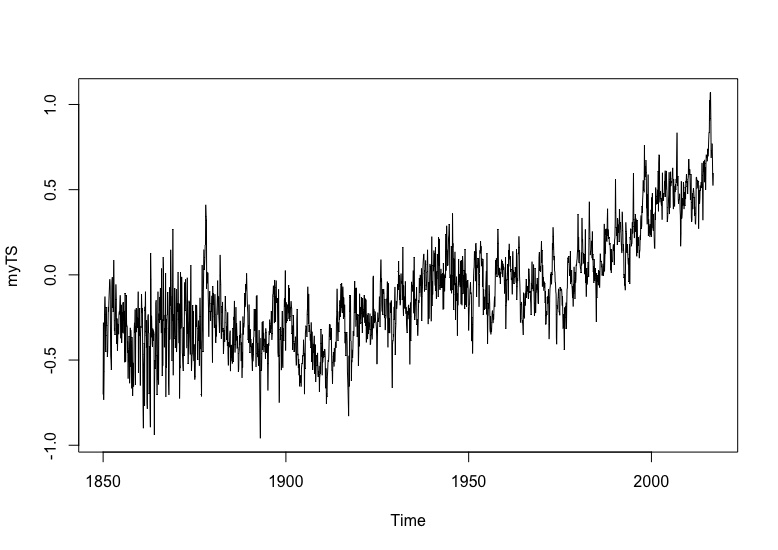
\includegraphics[scale=.5]{temp.png}
\end{figure}

\begin{figure}[H]
\centering
\caption{Plot myTS.adjusted}
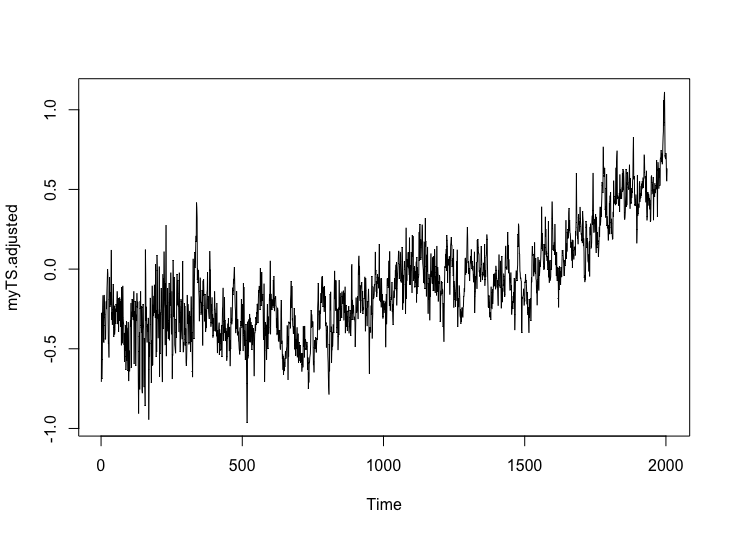
\includegraphics[scale=.5]{myTSadjusted.png}
\end{figure}


\subsubsection{ARIMA Model}
\begin{figure}[H]
\centering
\caption{Selecting arma order: acf of residuals of arma(2, 0, 1) \& (2, 1, 4)}
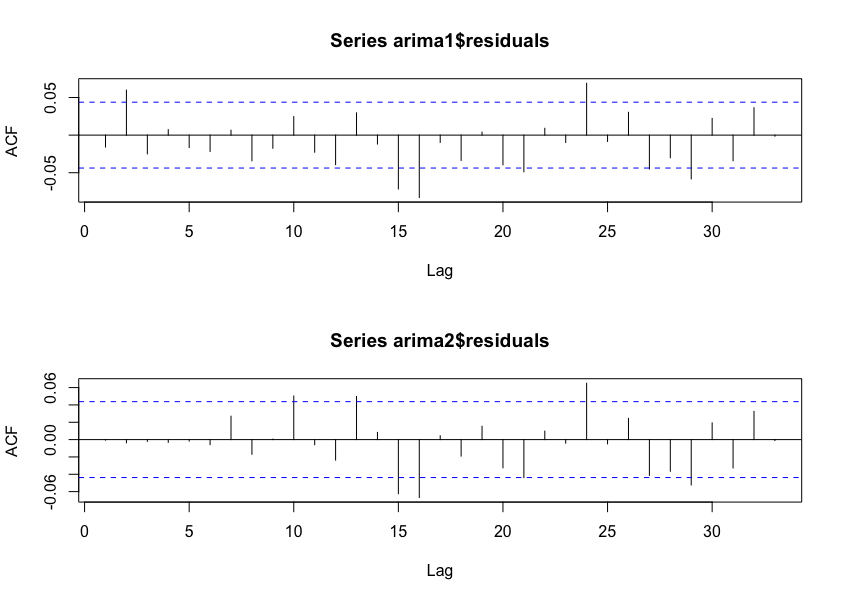
\includegraphics[scale=.5]{armaacf.png}
\end{figure}

\begin{figure}[H]
\centering
\caption{Selecting arma order: pacf of residuals of arma(2, 0, 1) \& (2, 1, 4)}
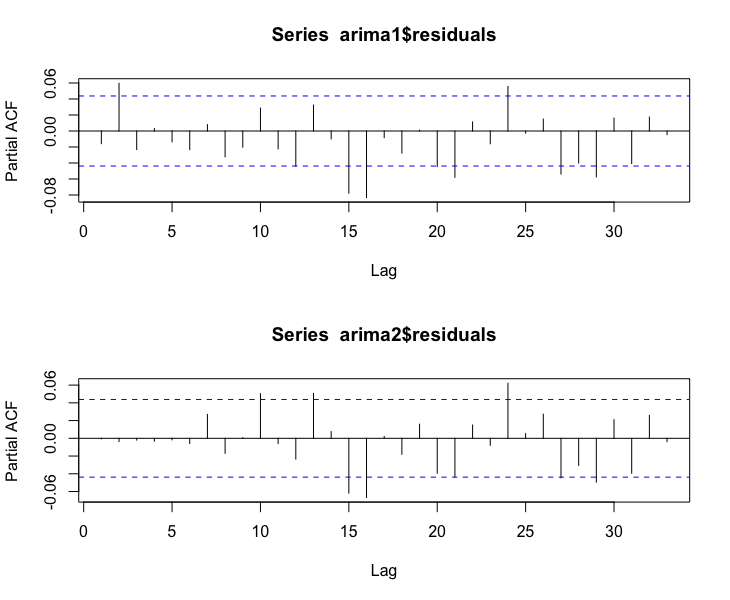
\includegraphics[scale=.5]{arima_pacf.png}
\end{figure}

\begin{figure}[H]
\centering
\caption{Forecast next 20 years(240 months) using arima(2, 1, 4)}
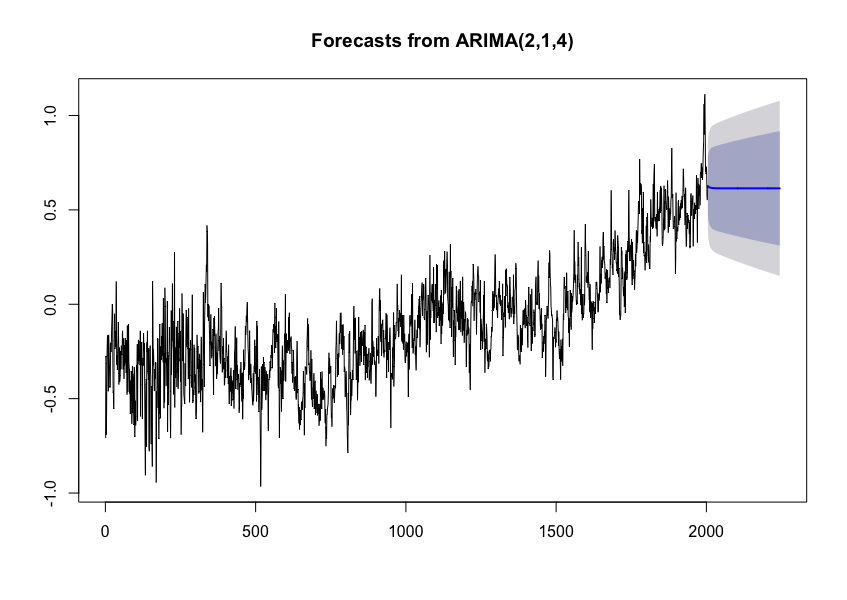
\includegraphics[scale=.5]{arima_forecast.png}
\end{figure}

\begin{figure}[H]
\centering
\caption{Forecast within the sample compared with the actual data using arima(2, 1, 4)}
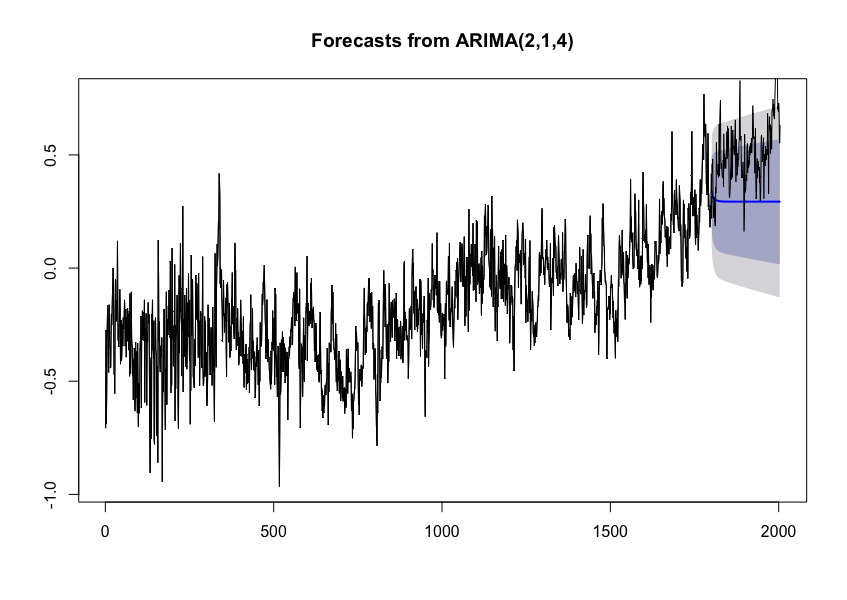
\includegraphics[scale=.5]{arima_sample.png}
\end{figure}


\subsubsection{ARFIMA Model}

\begin{figure}[H]
\centering
\caption{Plot arima2's residuals}
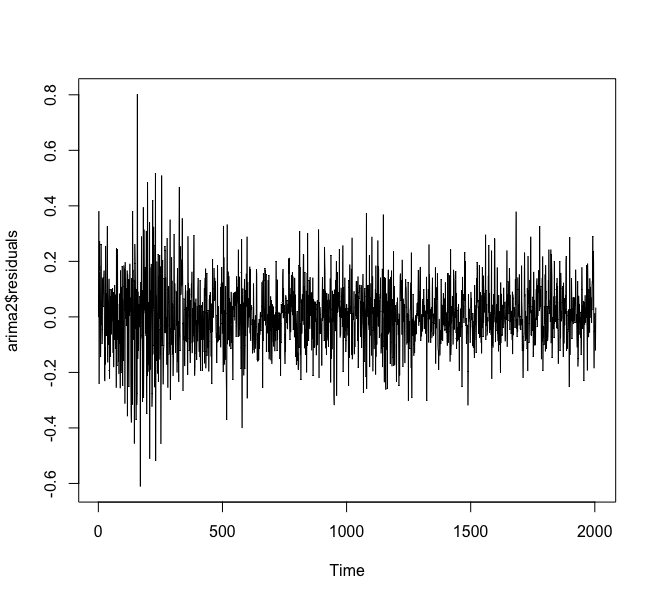
\includegraphics[scale=.5]{arima_residuals.png}
\end{figure}

\begin{figure}[H]
\centering
\caption{acf of residuals of ARFIMA}
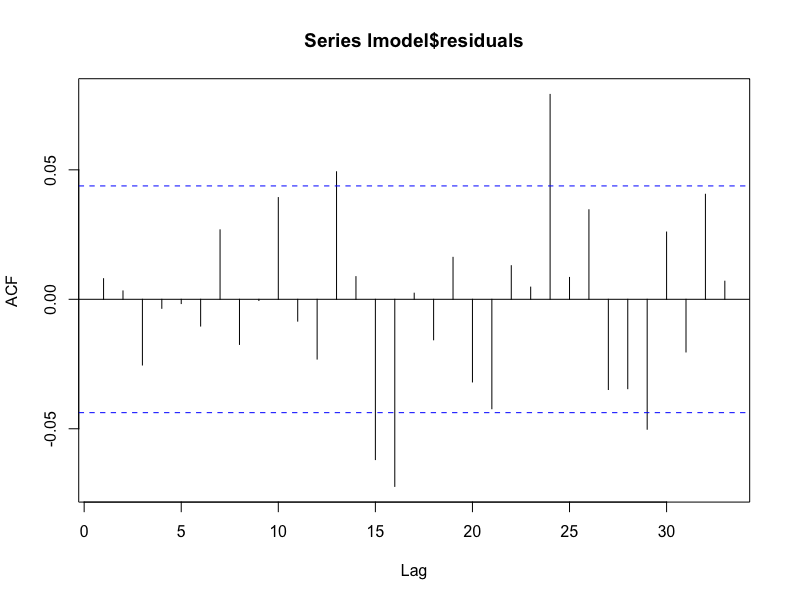
\includegraphics[scale=.5]{longacf.png}
\end{figure}


\subsubsection{More attempts on lag 24}
Original series' acf and pacf

\begin{figure}[H]
\centering
\caption{acf}
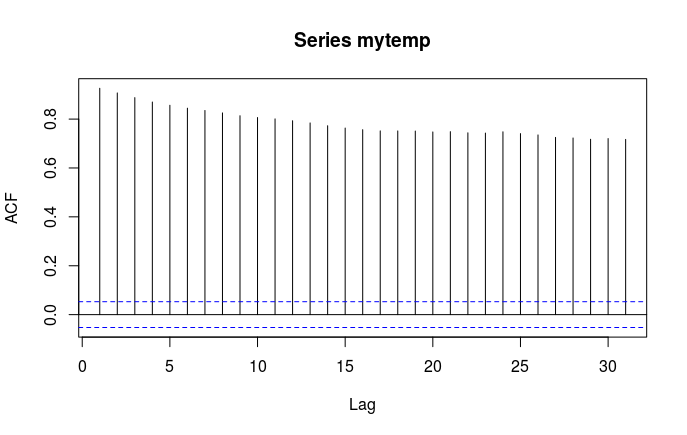
\includegraphics[scale=.70]{mytemp_acf.png}
\end{figure}

\begin{figure}[H]
\centering
\caption{pacf}
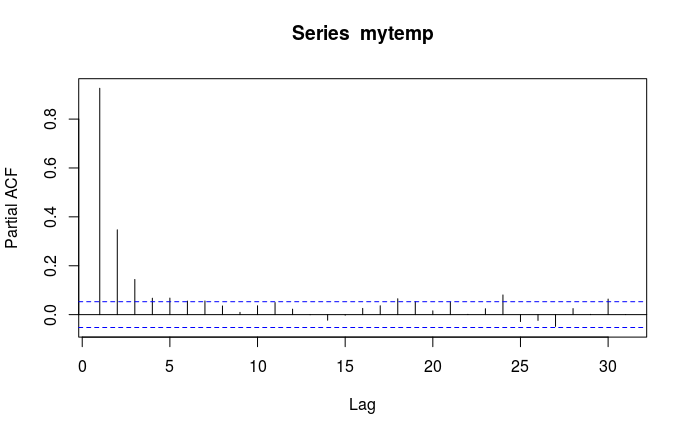
\includegraphics[scale=.70]{mytemp_pacf.png}
\end{figure}


\begin{figure}[H]
\centering
\caption{res2's acf}
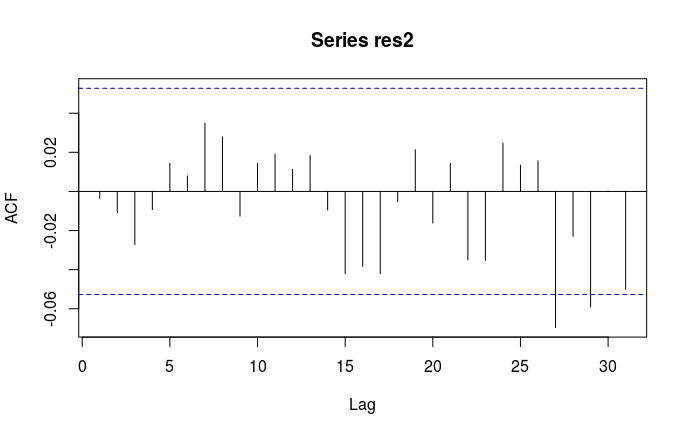
\includegraphics[scale=.70]{res2_acf.png}
\end{figure}

\begin{figure}[H]
\centering
\caption{res3's acf}
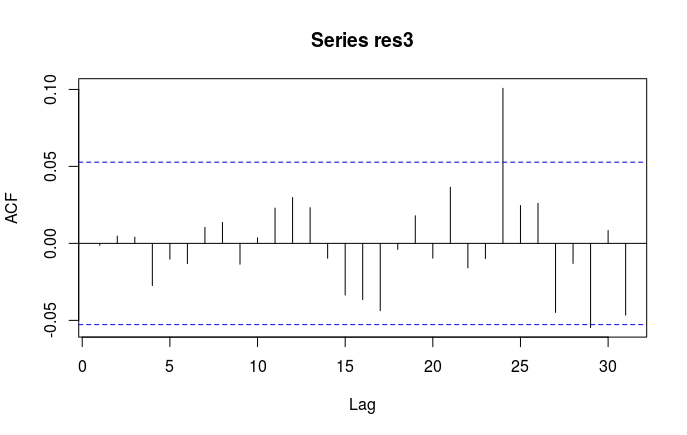
\includegraphics[scale=.70]{res3_acf.png}
\end{figure}



\begin{figure}[H]
\centering
\caption{final residuals: res4's acf}
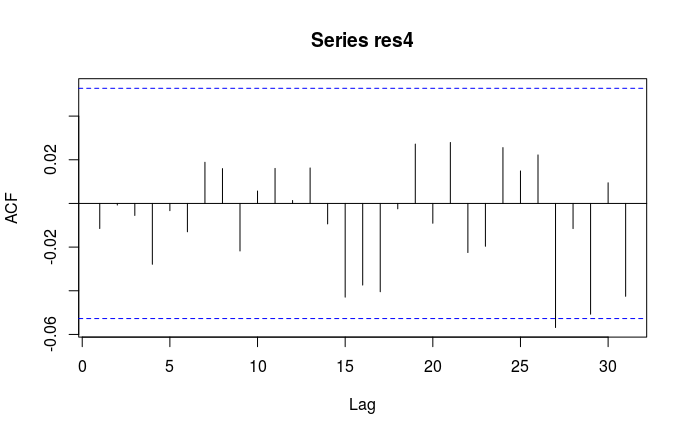
\includegraphics[scale=.70]{final_residuals_acf.png}
\end{figure}

The failure of trying pure seasonal adjustment

\begin{figure}[H]
\centering
\caption{res5's acf}
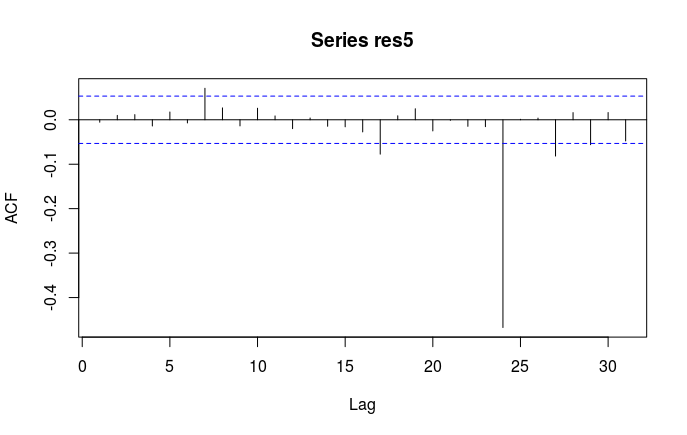
\includegraphics[scale=.70]{res5_acf.png}
\end{figure}


\subsubsection{GARCH Model}

\begin{figure}[H]
\centering
\caption{z}
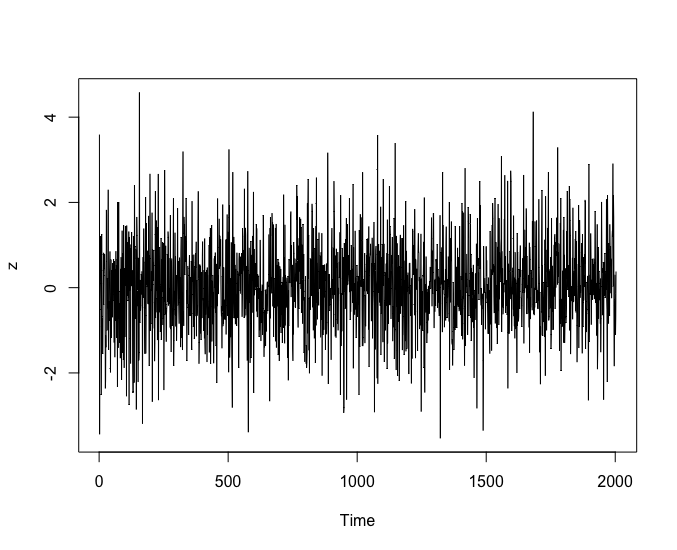
\includegraphics[scale=.40]{z.png}
\end{figure}

\begin{figure}[H]
\centering
\caption{simulation of using rnorm}
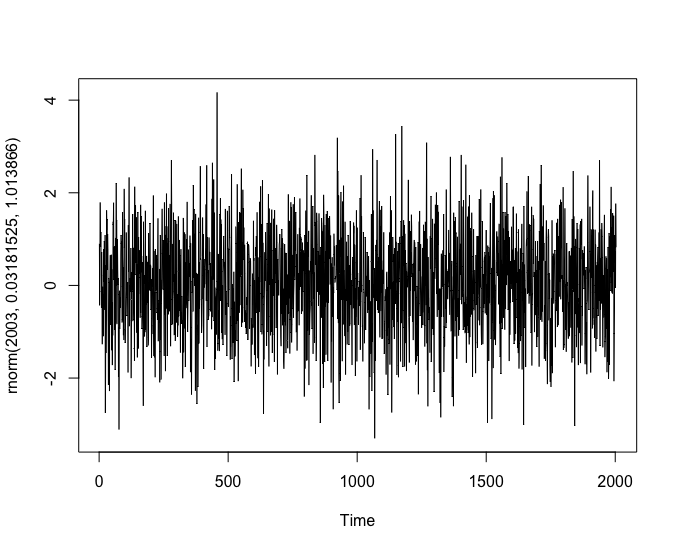
\includegraphics[scale=.40]{rnorm.png}
\end{figure}

\begin{figure}[H]
\centering
\caption{acf(z)}
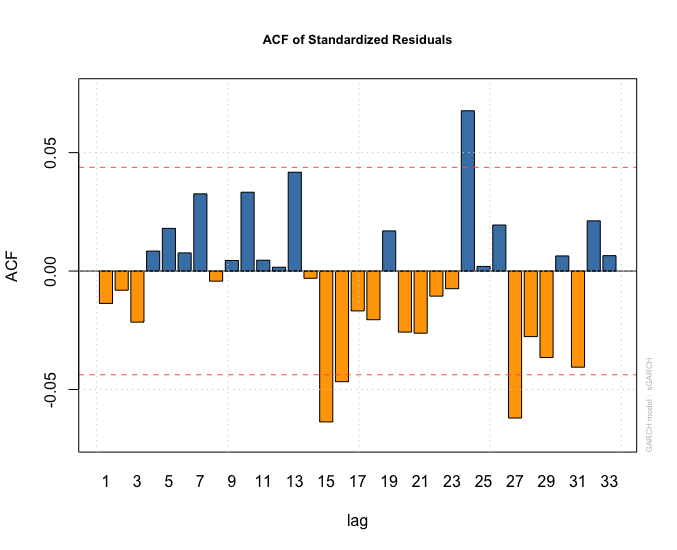
\includegraphics[scale=.50]{zacf.png}
\end{figure}

\begin{figure}[H]
\centering
\caption{Empirical Density of Standardized Residuals}
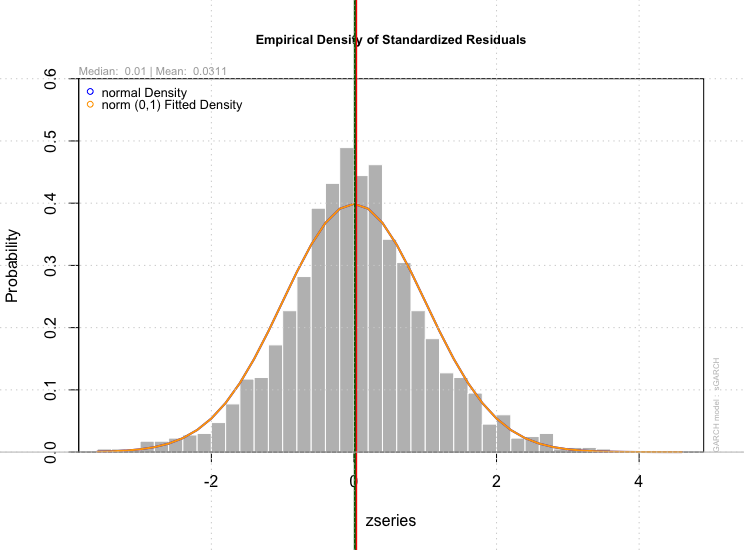
\includegraphics[scale=.50]{density.png}
\end{figure}
 

\begin{figure}[H]
\centering
\caption{qqplot of $z$}
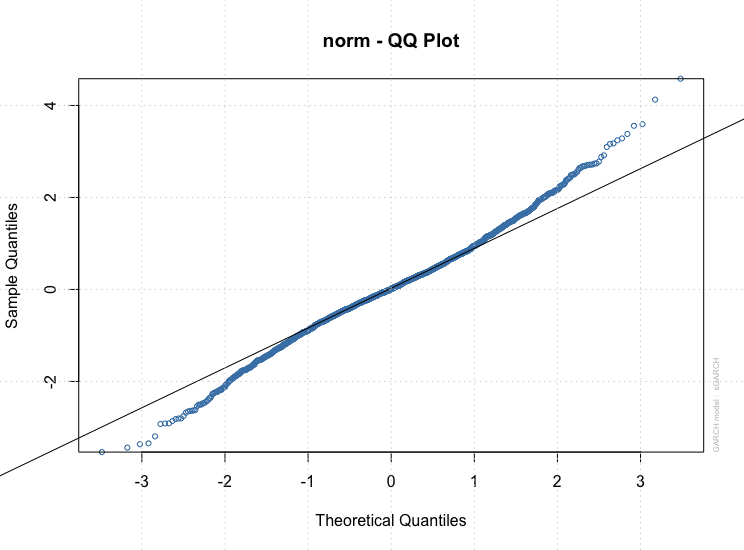
\includegraphics[scale=.50]{qqplot.png}
\end{figure}

\begin{figure}[H]
\centering
\caption{forecast for sGARCH Model}
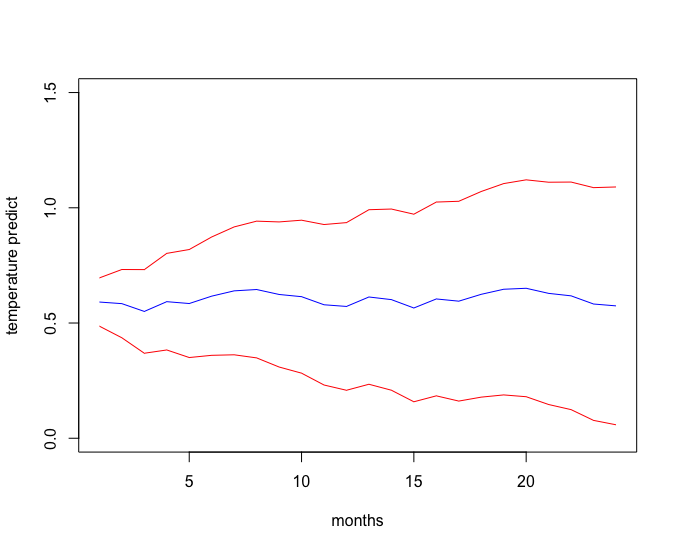
\includegraphics[scale=.50]{predict01.png}
\end{figure}

\subsubsection{CO2}


\begin{figure}[H]
\centering
\caption{ts.plot for diff(CO2)}
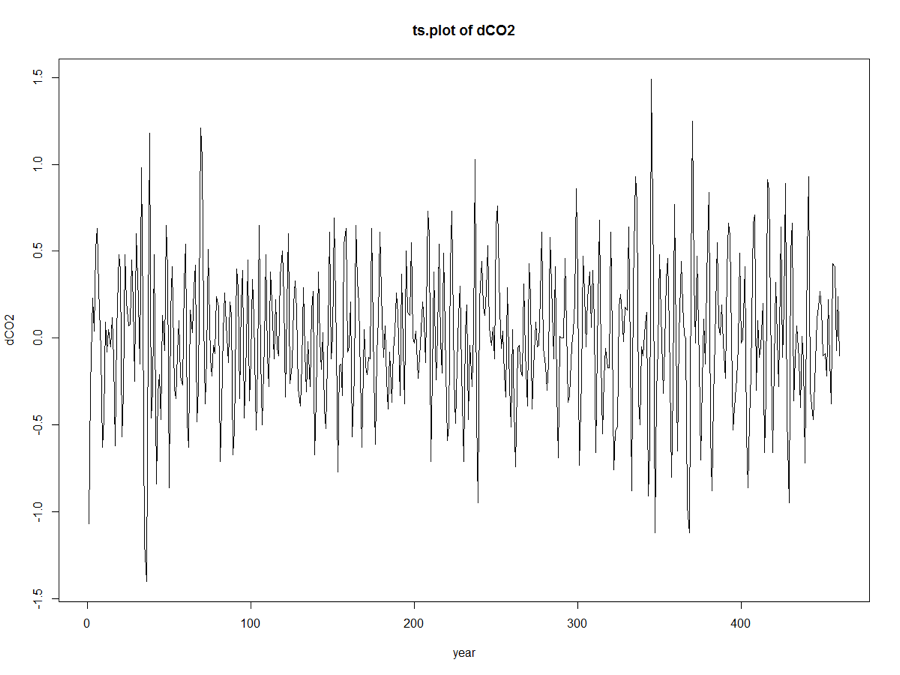
\includegraphics[scale=.80]{Picture1.png}
\end{figure}


\begin{figure}[H]
\centering
\caption{residuals of arima for CO2}
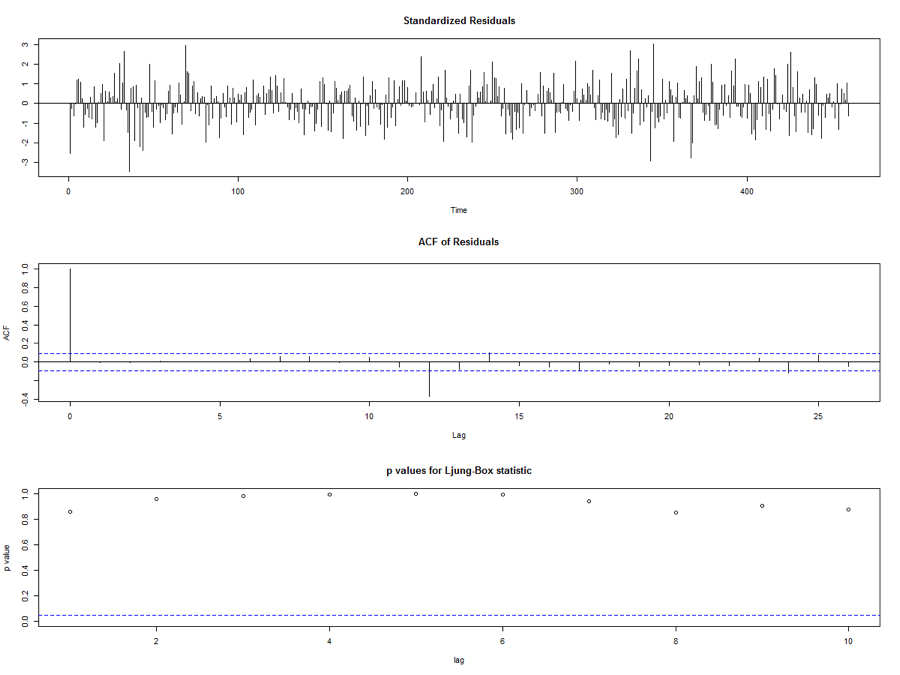
\includegraphics[scale=.80]{Picture2.png}
\end{figure}

\begin{figure}[H]
\centering
\caption{Seasonal effect of CO2 and temperature}
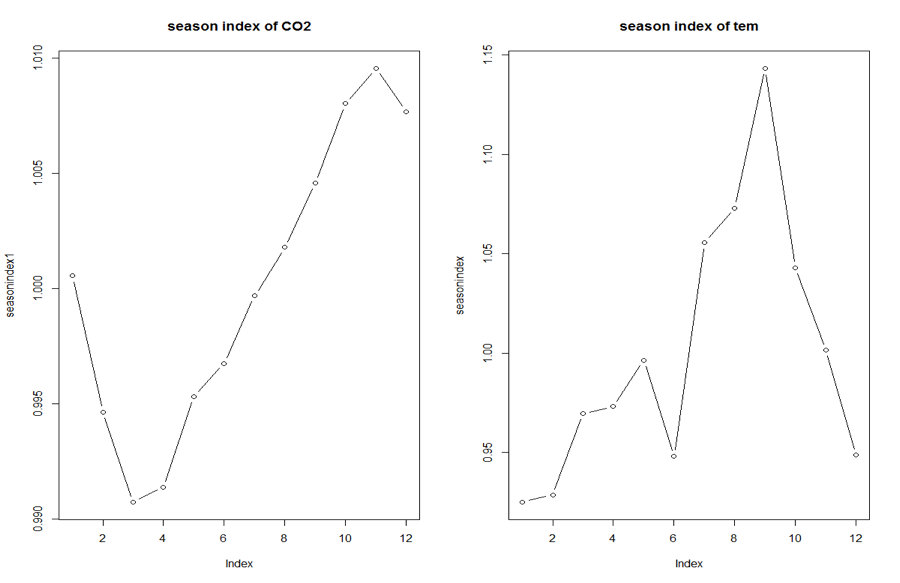
\includegraphics[scale=.80]{Picture3.png}
\end{figure}

\begin{figure}[H]
\centering
\caption{Timing diagram for CO2 and trend}
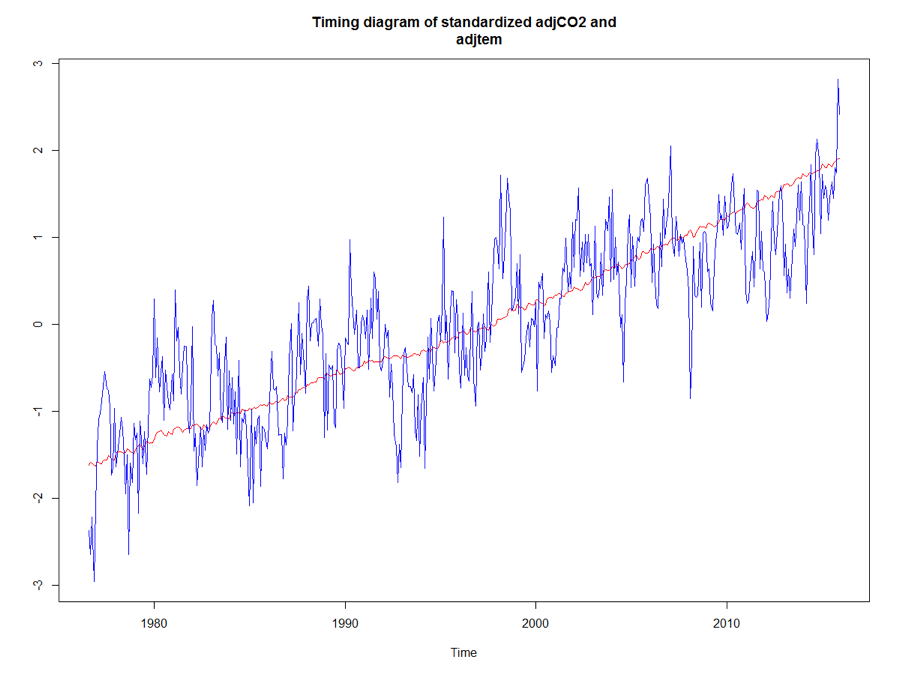
\includegraphics[scale=.80]{Picture4.png}
\end{figure}

\begin{figure}[H]
\centering
\caption{res2's acf}
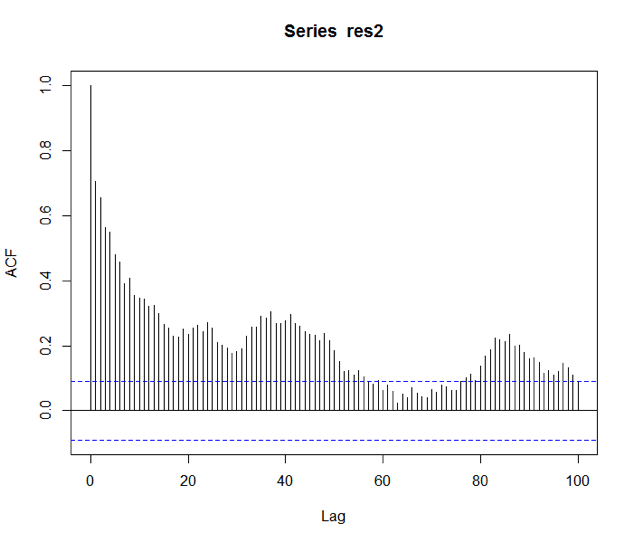
\includegraphics[scale=.80]{Picture5.png}
\end{figure}

\begin{figure}[H]
\centering
\caption{acf and pacf of residuals of Long-Memory Model}
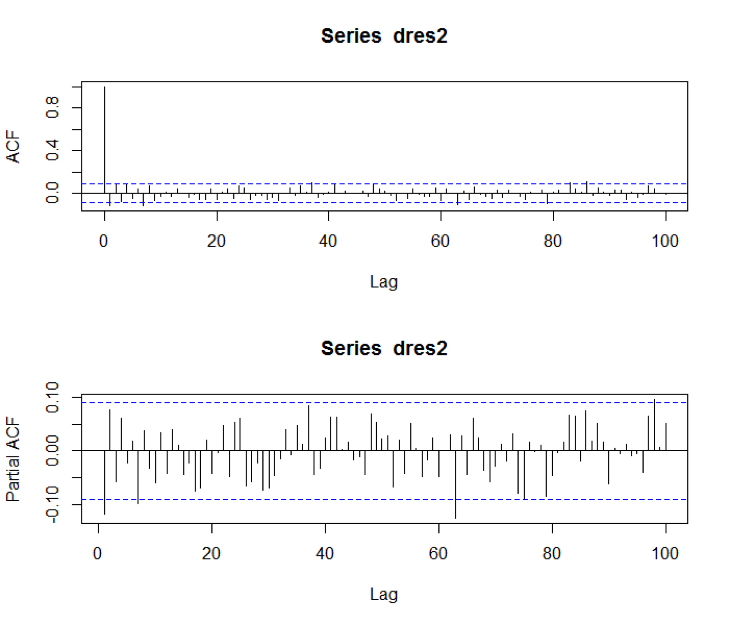
\includegraphics[scale=.80]{Picture6.png}
\end{figure}

\begin{figure}[H]
\centering
\caption{residuals of arima on dres2}
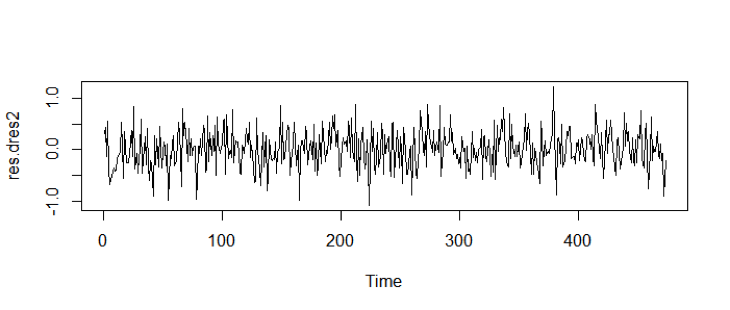
\includegraphics[scale=.80]{Picture7.png}
\end{figure}

\begin{figure}[H]
\centering
\caption{Timing diagram of res2}
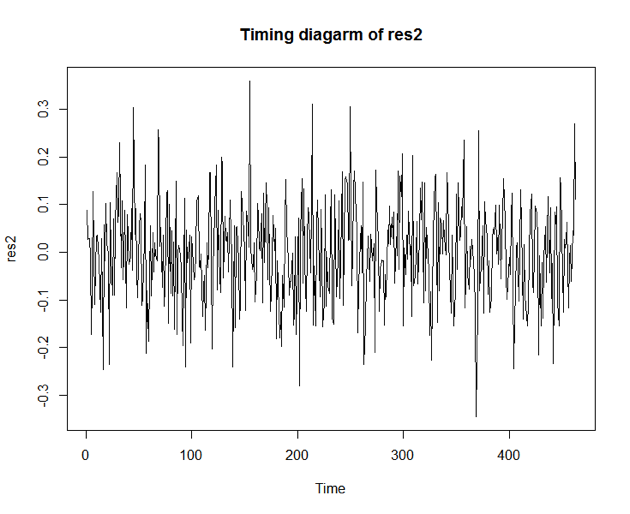
\includegraphics[scale=.80]{Picture8.png}
\end{figure}

\begin{figure}[H]
\centering
\caption{density plot and qqplot of res2}
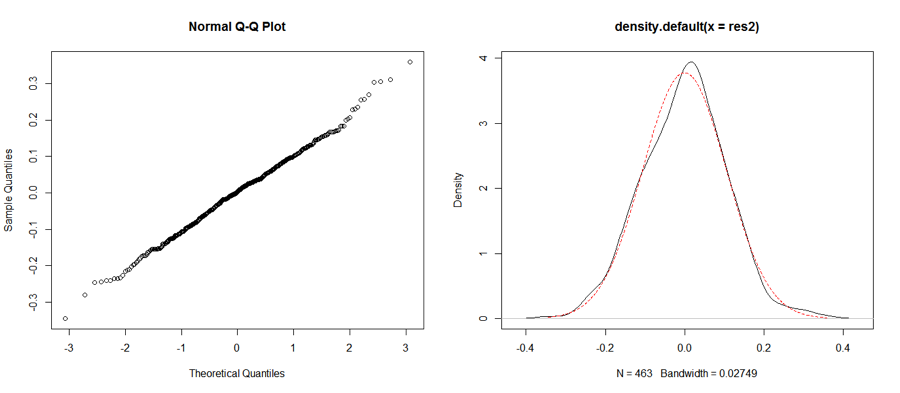
\includegraphics[scale=.80]{Picture9.png}
\end{figure}

\begin{figure}[H]
\centering
\caption{fitting diagram of the model}
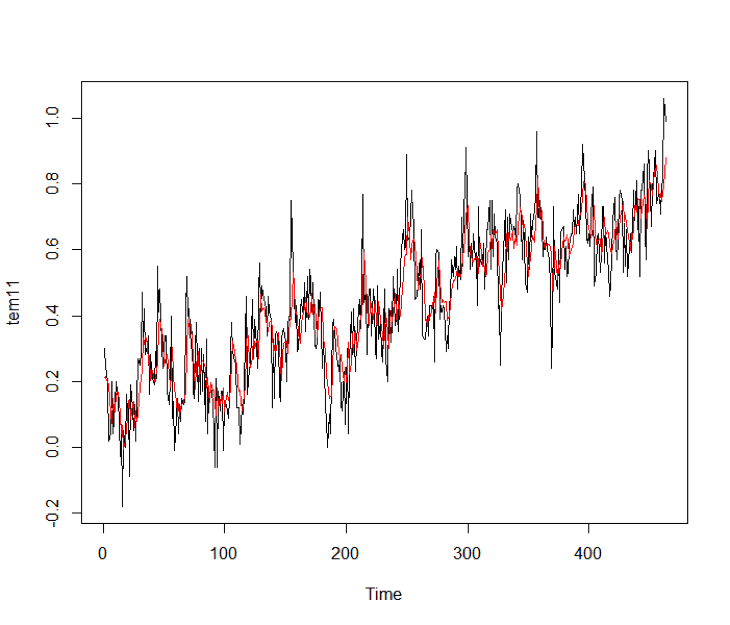
\includegraphics[scale=.80]{Picture10.png}
\end{figure}

\begin{figure}[H]
\centering
\caption{res4}
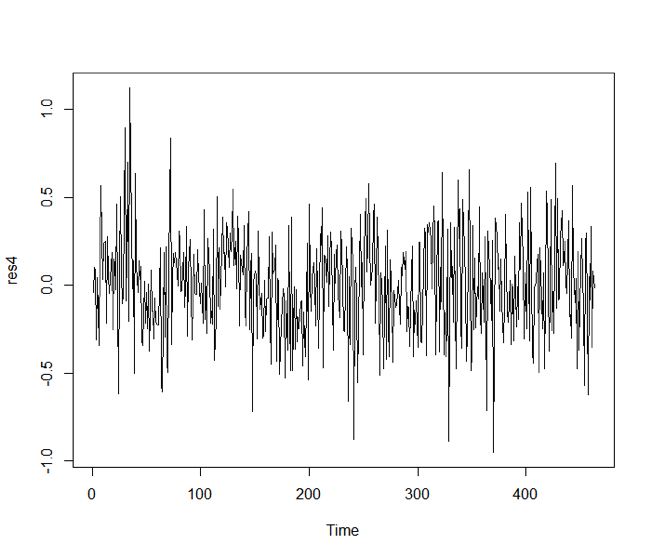
\includegraphics[scale=.80]{Picture11.png}
\end{figure}

\begin{figure}[H]
\centering
\caption{res4's acf and pacf}
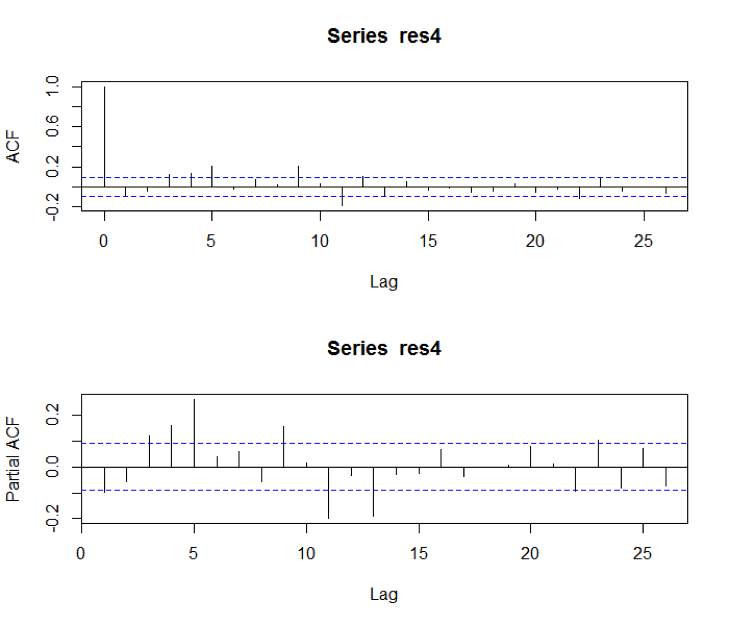
\includegraphics[scale=.80]{Picture12.png}
\end{figure}

\begin{figure}[H]
\centering
\caption{Timing diagram of dres4}
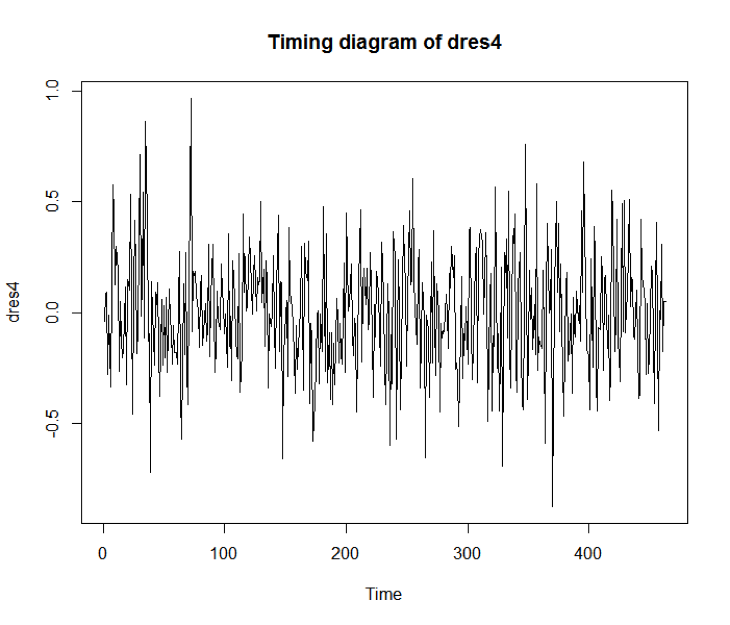
\includegraphics[scale=.80]{Picture13.png}
\end{figure}

\begin{figure}[H]
\centering
\caption{density of dres4}
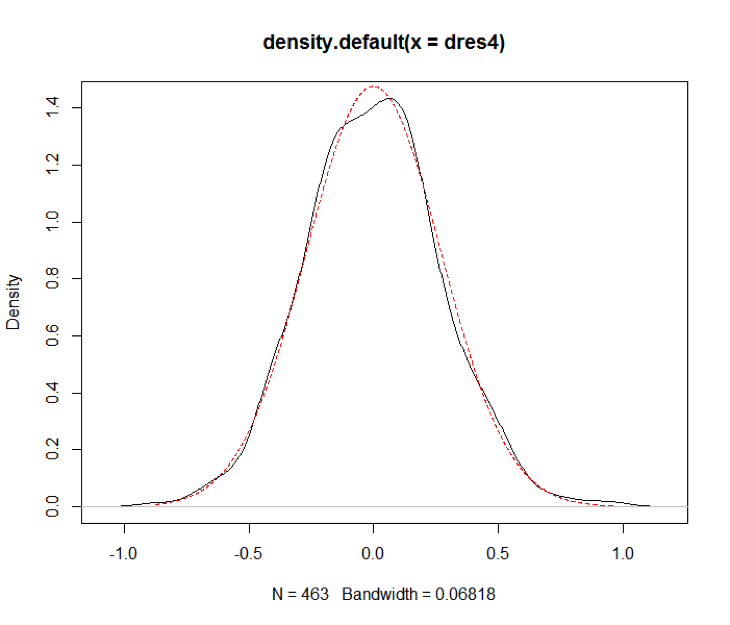
\includegraphics[scale=.80]{Picture14.png}
\end{figure}




\subsection{Others}
\subsubsection{Details about \textit{decompose()} used in seasonal adjustment}
Type `decompose' in R console, we can see the source code of this function. The process of `type = additive' is listed below:
\begin{itemize}
\item the argument passed into decompose() is a `ts' object 
\item denote the argument ts(x, frequency = f). Create a filter using: filter = c(0.5, rep(1, f - 1), 0.5)/f.
\item trend = filter(x, filter)
\item season = x - trend, then compute f means of season with interval length f, the f means denoted by figure. Adjusting figure figure = figure - mean(figure)
\item seasonal is just length(x)/f times repetition of figure.
\item random = x - seasonal - trend
\end{itemize}


\end{document}